\section{Getting Started with JAX-WS Web Services}
This lab demonstrates the basics of using the IDE to develop a JAX-WS web service. After you create the web service, you write three different web service clients that use the web service over a network, which is called "consuming" a web service. The three clients are a Java class in a Java SE application, a servlet, and a JSP page in a web application. 
\subsection{Creating a Web Service}
The goal of this exercise is to create a project appropriate to the deployment container that you decide to use. Once you have a project, you will create a web service in it.
\subsubsection{Choosing a Container}
Create a web application.
\begin{enumerate}
\item Choose File > New Project (Ctrl-Shift-N on Linux and Windows). Select Web Application from the Java Web category or EJB Module from the Java EE category.
\item Name the project \texttt{CalculatorWSApplication}. Select a location for the project. Click Next. 
\item Select your server and Java EE version and click Finish.
\end{enumerate}
\subsubsection{Creating a Web Service from a Java Class}
\begin{enumerate}
\item Right-click the CalculatorWSApplication node and choose New > Web Service.
\item Name the web service CalculatorWS and type org.me.calculator in Package. Leave Create Web Service from Scratch selected.
\item If you are creating a Java EE 6 project on GlassFish or WebLogic, select Implement Web Service as a Stateless Session Bean.

\begin{figure}
\begin{center}
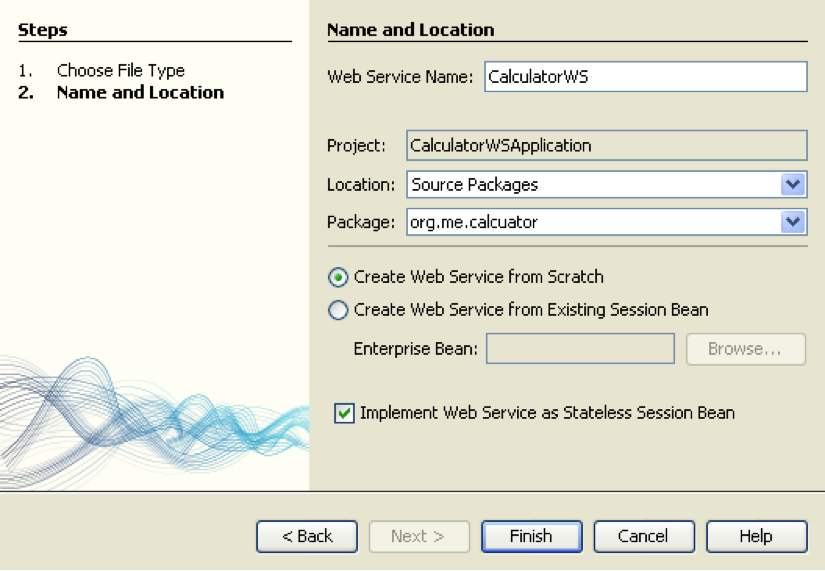
\includegraphics[scale=1]{J1}
%\caption{Objects encapsulate data and behavior}
\label{J1}
\end{center}
\end{figure}

\item Click Finish. The Projects window displays the structure of the new web service and the source code is shown in the editor area.
\end{enumerate}

\subsection{Adding an Operation to the Web Service}
The goal of this exercise is to add to the web service an operation that adds two numbers received from a client. The NetBeans IDE provides a dialog for adding an operation to a web service. 
\subsubsection{To add an operation to the web service:}
\begin{enumerate}
\item Either:
\begin{itemize}
\item Change to the Design view in the editor.

\begin{figure}
\begin{center}
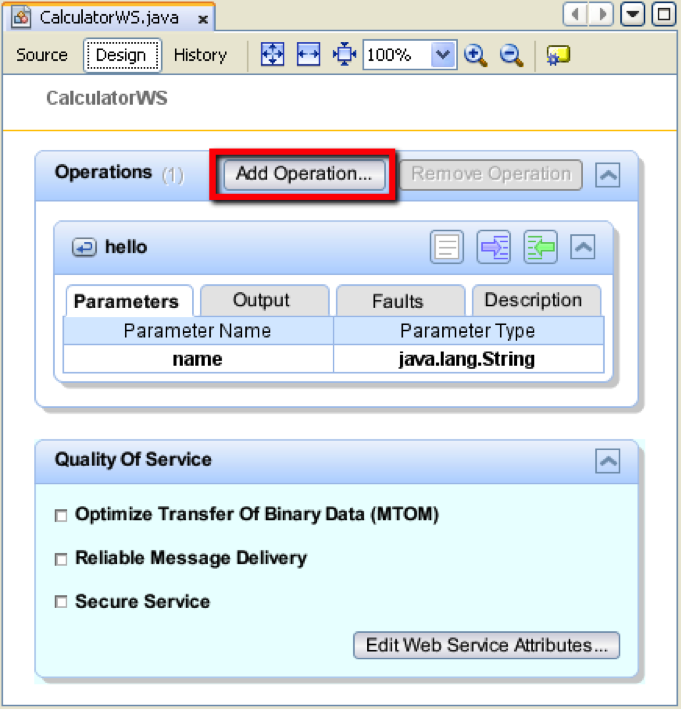
\includegraphics[scale=1]{J2}
%\caption{Objects encapsulate data and behavior}
\label{J2}
\end{center}
\end{figure}

\item Or: Find the web service's node in the Projects window. Right-click that node. A context menu opens.

\begin{figure}
\begin{center}
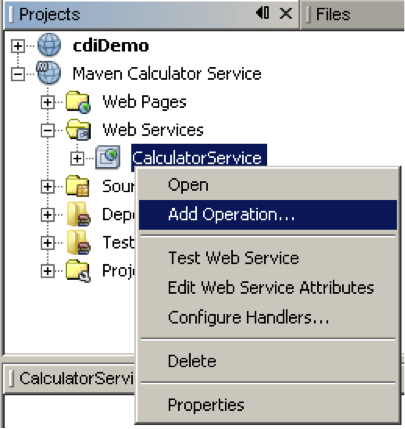
\includegraphics[scale=1]{J3}
%\caption{Objects encapsulate data and behavior}
\label{J3}
\end{center}
\end{figure}

\end{itemize}
\item Click Add Operation in either the visual designer or the context menu. The Add Operation dialog opens.
\item In the upper part of the Add Operation dialog box, type add in Name and type int in the Return Type drop-down list.
\item In the lower part of the Add Operation dialog box, click Add and create a parameter of type int named i.
\item Click Add again and create a parameter of type int called j.
You now see the following:

\begin{figure}
\begin{center}
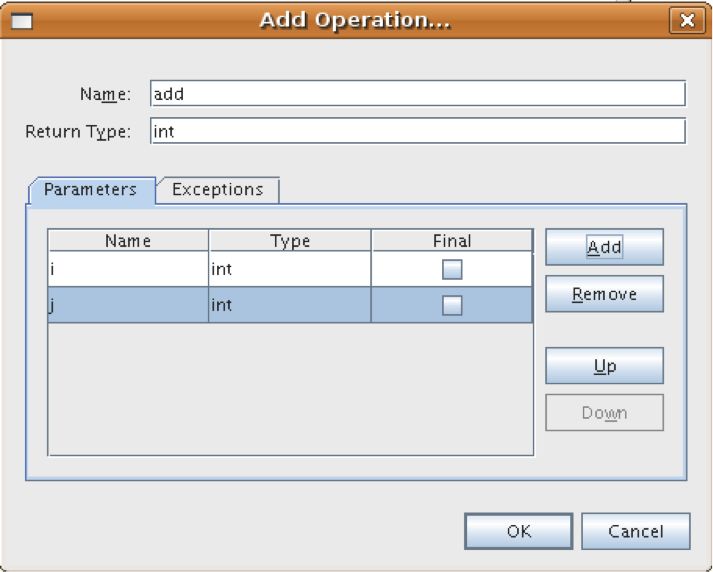
\includegraphics[scale=1]{J4}
%\caption{Objects encapsulate data and behavior}
\label{J4}
\end{center}
\end{figure}

\item Click OK at the bottom of the Add Operation dialog box. You return to the editor.
\item Remove the default hello operation, either by deleting the hello() method in the source code or by selecting the hello operation in the visual designer and clicking Remove Operation.
The visual designer now displays the following:

\begin{figure}
\begin{center}
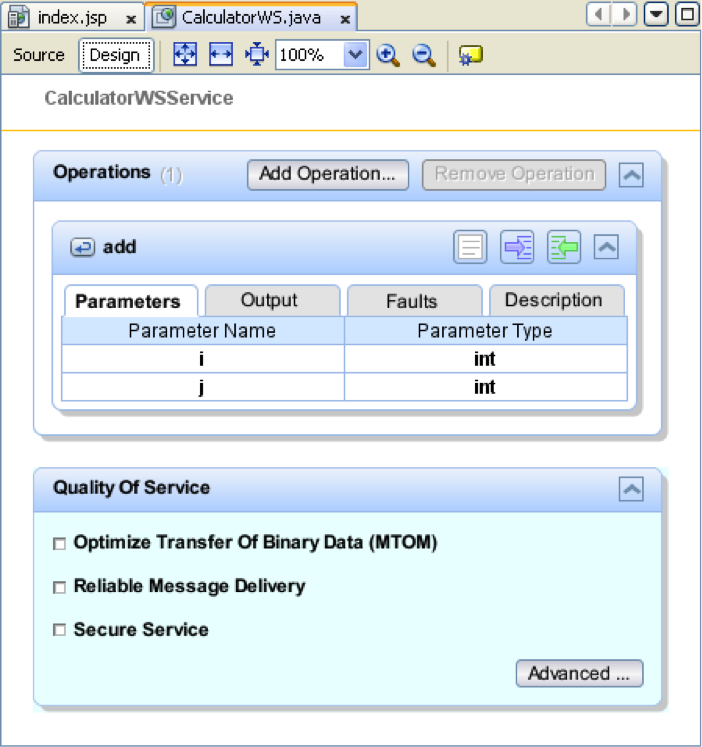
\includegraphics[scale=1]{J5}
%\caption{Objects encapsulate data and behavior}
\label{J5}
\end{center}
\end{figure}

\item Click Source and view the code that you generated in the previous steps. 

\begin{figure}
\begin{center}
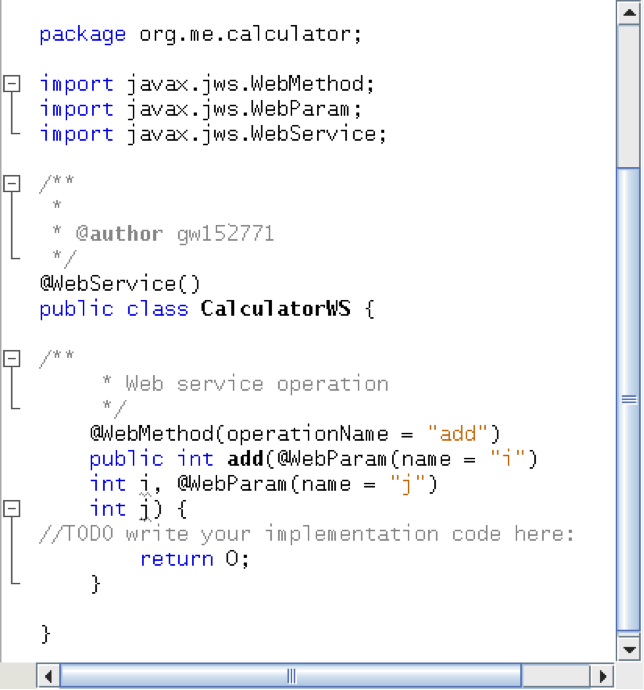
\includegraphics[scale=1]{J6}
%\caption{Objects encapsulate data and behavior}
\label{J6}
\end{center}
\end{figure}

\begin{figure}
\begin{center}
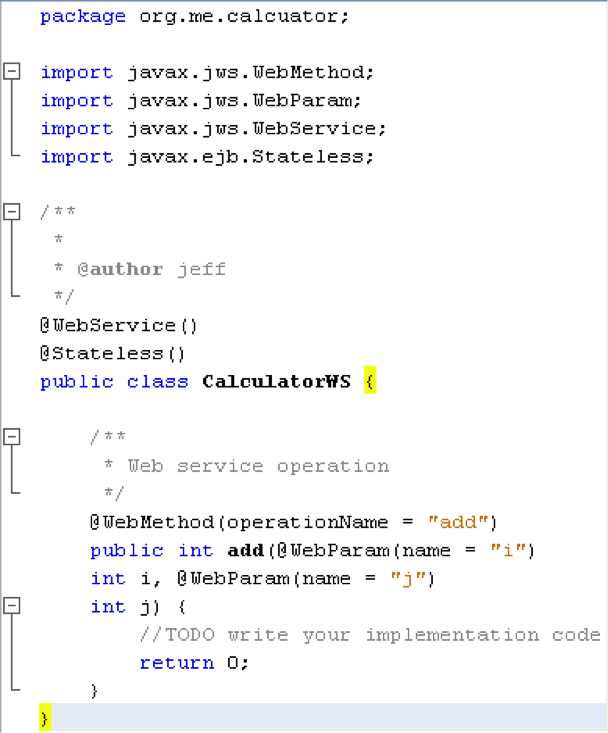
\includegraphics[scale=1]{J7}
%\caption{Objects encapsulate data and behavior}
\label{J7}
\end{center}
\end{figure}

\item In the editor, extend the skeleton add operation to the following (changes are in bold):

\begin{lstlisting}
@WebMethod
    public int add(@WebParam(name = "i") int i, @WebParam(name = "j") int j) {
        int k = i + j;
        return k;
      }
\end{lstlisting}

As you can see from the preceding code, the web service simply receives two numbers and then returns their sum. In the next section, you use the IDE to test the web service.
\end{enumerate}

\section{Deploying and Testing the Web Service}
After you deploy a web service to a server, you can use the IDE to open the server's test client, if the server has a test client. The GlassFish and WebLogic servers provide test clients.

To test successful deployment to a GlassFish or WebLogic server:
\begin{enumerate}
\item Right-click the project and choose Deploy. The IDE starts the application server, builds the application, and deploys the application to the server. You can follow the progress of these operations in the CalculatorWSApplication (run-deploy) and the GlassFish server or Tomcat tabs in the Output view.
\item In the IDE's Projects tab, expand the Web Services node of the CalculatorWSApplication project. Right-click the CalculatorWS node, and choose Test Web Service.
\end{enumerate}

\begin{figure}
\begin{center}
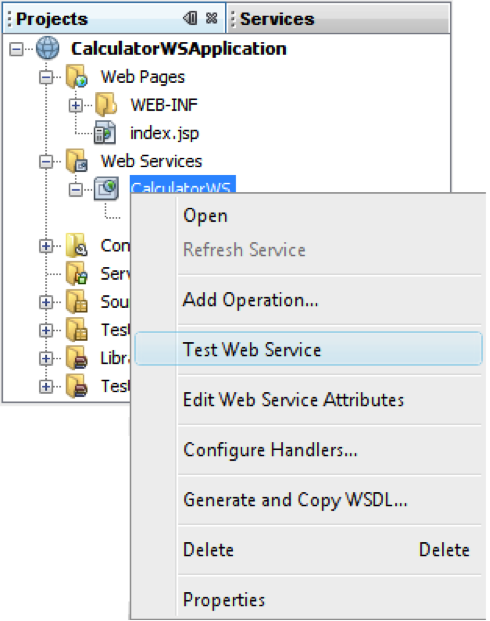
\includegraphics[scale=1]{J8}
%\caption{Objects encapsulate data and behavior}
\label{J8}
\end{center}
\end{figure}

The IDE opens the tester page in your browser, if you deployed a web application to the GlassFish server.
\begin{itemize}
\item If you deployed to the GlassFish server, type two numbers in the tester page, as shown below:

\begin{figure}
\begin{center}
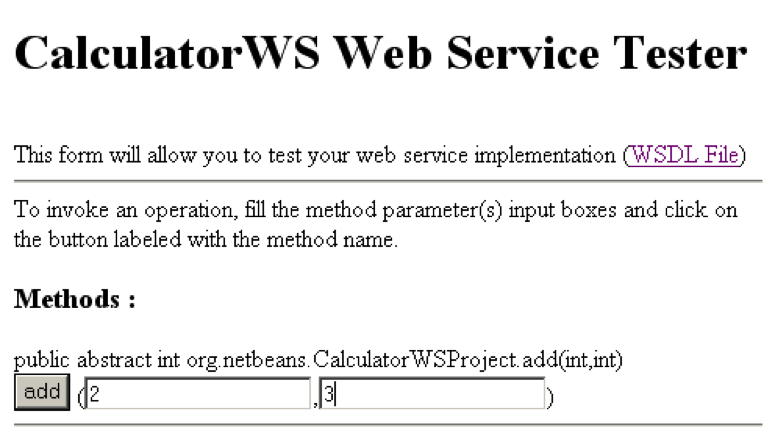
\includegraphics[scale=1]{J9}
%\caption{Objects encapsulate data and behavior}
\label{J9}
\end{center}
\end{figure}

\item The sum of the two numbers is displayed:

\begin{figure}
\begin{center}
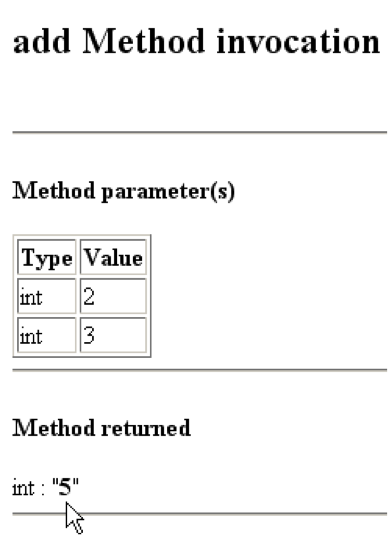
\includegraphics[scale=1]{J10}
%\caption{Objects encapsulate data and behavior}
\label{J10}
\end{center}
\end{figure}

\end{itemize}

\section{Consuming the Web Service}
Now that you have deployed the web service, you need to create a client to make use of the web service's add method. Here, you create three clients— a Java class in a Java SE application, a servlet, and a JSP page in a web application.

\subsection{Client 1: Java Class in Java SE Application}
In this section, you create a standard Java application. The wizard that you use to create the application also creates a Java class. You then use the IDE's tools to create a client and consume the web service that you created at the start of this tutorial.
\begin{enumerate}
\item Choose File > New Project (Ctrl-Shift-N on Linux and Windows). Select Java Application from the Java category. Name the project CalculatorWS_Client_Application. Leave Create Main Class selected and accept all other default settings. Click Finish.
\item Right-click the CalculatorWS_Client_Application node and choose New > Web Service Client. The New Web Service Client wizard opens. 
\item Select Project as the WSDL source. Click Browse. Browse to the CalculatorWS web service in the CalculatorWSApplication project. When you have selected the web service, click OK.

\begin{figure}
\begin{center}
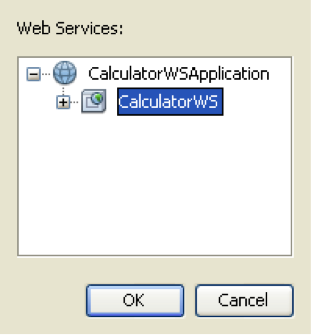
\includegraphics[scale=1]{J11}
%\caption{Objects encapsulate data and behavior}
\label{J11}
\end{center}
\end{figure}

\item Do not select a package name. Leave this field empty.

\begin{figure}
\begin{center}
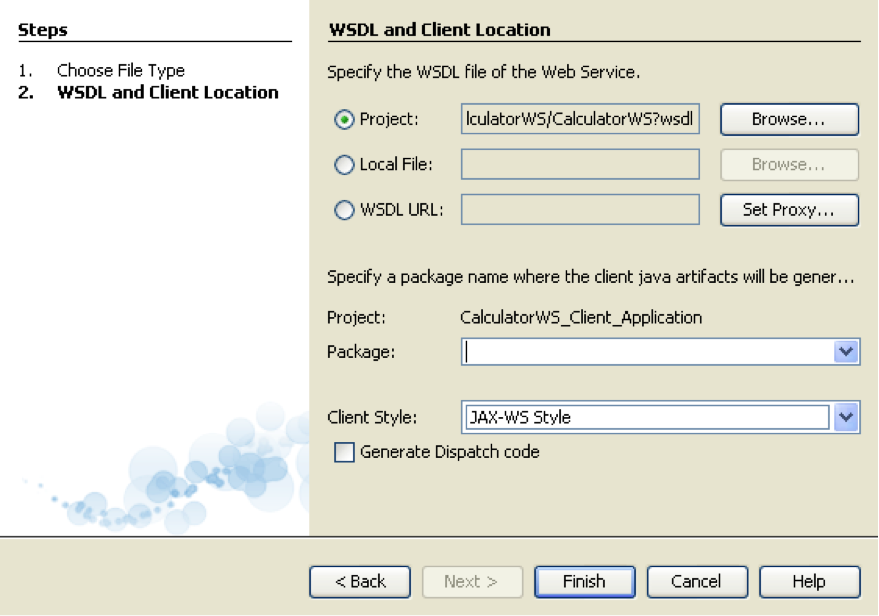
\includegraphics[scale=1]{J12}
%\caption{Objects encapsulate data and behavior}
\label{J12}
\end{center}
\end{figure}

\item Leave the other settings at default and click Finish.
The Projects window displays the new web service client, with a node for the add method that you created:

\begin{figure}
\begin{center}
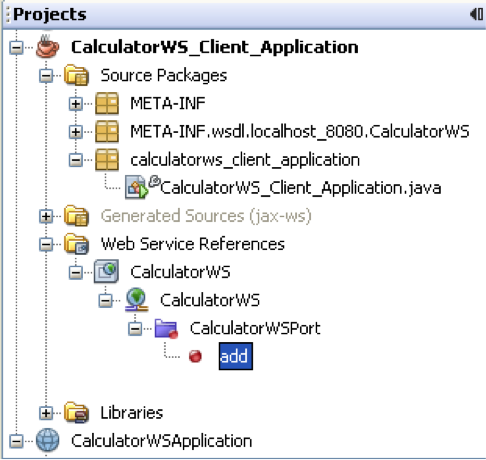
\includegraphics[scale=1]{J13}
%\caption{Objects encapsulate data and behavior}
\label{J13}
\end{center}
\end{figure}

\item Double-click your main class so that it opens in the Source Editor. Drag the add node below the main() method.

\begin{figure}
\begin{center}
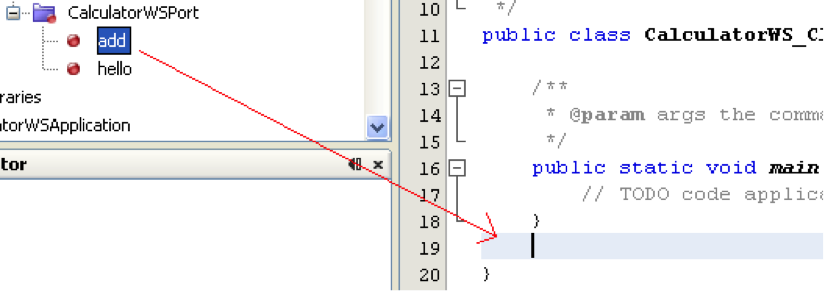
\includegraphics[scale=1]{J14}
%\caption{Objects encapsulate data and behavior}
\label{J14}
\end{center}
\end{figure}

You now see the following:
\begin{lstlisting}
public static void main(String[] args) {
    // TODO code application logic here
}
private static int add(int i, int j) {
    org.me.calculator.CalculatorWS_Service service = new org.me.calculator.CalculatorWS_Service();
    org.me.calculator.CalculatorWS port = service.getCalculatorWSPort();
    return port.add(i, j);
}
\end{lstlisting}
Note: Alternatively, instead of dragging the add node, you can right-click in the editor and then choose Insert Code > Call Web Service Operation. 

\item In the main() method body, replace the TODO comment with code that initializes values for i and j, calls add(), and prints the result.
\begin{lstlisting}
public static void main(String[] args) {
    int i = 3;
    int j = 4;
    int result = add(i, j);
    System.out.println("Result = " + result);
}
\end{lstlisting}

\item Surround the main() method code with a try/catch block that prints an exception. 
\begin{lstlisting}
public static void main(String[] args) {
    try {
        int i = 3;
        int j = 4;
        int result = add(i, j);
        System.out.println("Result = " + result);
    } catch (Exception ex) {
        System.out.println("Exception: " + ex);
    }
}
\end{lstlisting}

\item 10.	Right-click the project node and choose Run.
The Output window now shows the sum:
\begin{lstlisting}
compile:
    run:
    Result = 7
      BUILD SUCCESSFUL (total time: 1 second)
\end{lstlisting}

\subsection{Client 2: Servlet in Web Application}
In this section, you create a new web application, after which you create a servlet. You then use the servlet to consume the web service that you created at the start of this tutorial.
\begin{enumerate}
\item Choose File > New Project (Ctrl-Shift-N on Linux and Windows). Select Web Application from the Java Web category. Name the project CalculatorWSServletClient. Click Next and then click Finish.
\item Right-click the CalculatorWSServletClient node and choose New > Web Service Client.
The New Web Service Client wizard appears.
\item Select Project as the WSDL source. Click Browse. Browse to the CalculatorWS web service in the CalculatorWSApplication project. When you have selected the web service, click OK.

\begin{figure}
\begin{center}
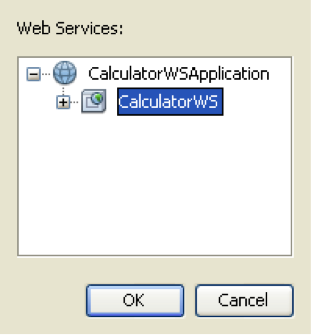
\includegraphics[scale=1]{J15}
%\caption{Objects encapsulate data and behavior}
\label{J15}
\end{center}
\end{figure}

\item Do not select a package name. Leave this field empty.
\item Leave the other settings at default and click Finish.
The Web Service References node in the Projects window displays the structure of your newly created client, including the add operation that you created earlier in this tutorial:

\begin{figure}
\begin{center}
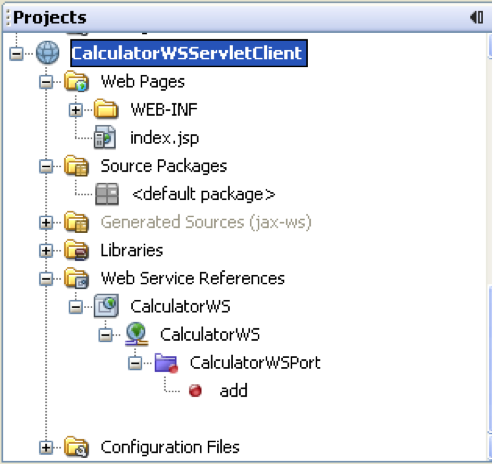
\includegraphics[scale=1]{J16}
%\caption{Objects encapsulate data and behavior}
\label{J16}
\end{center}
\end{figure}

\item Right-click the CalculatorWSServletClient project node and choose New > Servlet. Name the servlet ClientServlet and place it in a package called org.me.calculator.client. Click Finish.

